\section{Experiments}
% which experiements will we do on our model?
	% List them - gør det overskueligt!!!
	
% Hvad vil det sige at predicte en helix
% Skal hver position have den rigtige klasse
% Skal den ses som et samlet strykke af positioner med samme klasse.
% i så fald hvornår er den rigtig.
% Vi har brugt to forskellige mål for hvornår en prediction er rigtig
% Den første kræver 50% overlap og ender inden for 5 position for at den gælder som rigtig
% Den anden kræver kun 25% overlap

	
% The results we allready have of the other model - or the tests we need to do, to be able to compare the models.
% the data used

% Hvad forventer vi resultaterne vil være.

All the weights and biases in the model gets initialized by random values and the training
is done by mini-batch gradient descent, where a random batch of the samples is used to 
calculate the gradient. The training can converge to different local minima with 
different initial variables and order of batches.
The trained model is therefore very sensitive to the initial assignment of 
variables and the order the samples is used. It is therefore unlikely to get the same 
result every time the model is trained and can have a very high variance. 
Each experiment was therefore run ten times and the mean was used as result with 
the standard deviation of these runs as error rates.


\subsection{Dataset}
The dataset used to train and test the model is the TMP166\cite{tmseg} dataset used to 
develop TMSEG. The dataset consists of four subsets with approximate the same distribution 
of different length of proteins. The fourth subset was omitted from the training and only 
used to test the final model on. This was done to be sure that the model was not overfitted
on the test set and that the model was generalizing to new data. 

\subsection{Training}
\glspl{lstm} is fairly slow in terms of time, both to inference and especially to train.
This is because \gls{lstm} layers needs lots of computations in comparison with ordinary 
fully connected layers and most \glspl{ann} is already slow in comparison with many 
other types of machine learning.
\todo{maybe some timing test and comparison with HMM}

Proper grid search of hyper-parameters is a very long process because the time it takes
scales exponential in the number of different hyper-parameters and the model has a lot 
of them and together with the fairly long training time is the whole process very slow.
I have therefore chosen not to do a complete grid search,
but a more linear approach where it goes through the hyper-parameters one at a time and
tries different values and chooses the one that gives the best average precision and recall.
It then goes through the hyper-parameters again to see if different values a better in 
combination with the values chosen later in the process.
The standard deviation was some times bigger than the difference of to values for some 
of the parameters, therefore was each value used in a 3-fold cross-validation on the 
three first subsets, this way it was more consistent which value was the best for a 
given hyper-parameter.

\begin{figure}
	\centering
	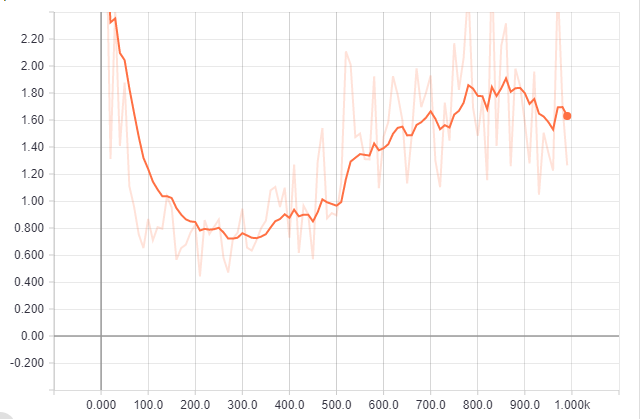
\includegraphics[width=\textwidth]{sections/experiments/overfitting}
	\caption{The development of the step 1 loss function on the validation set over the training.
	shows clear signs of overfitting. Smoothed to make the trend more clear.}
	\label{fig:overfitting}
\end{figure}

\begin{figure}
	\centering
	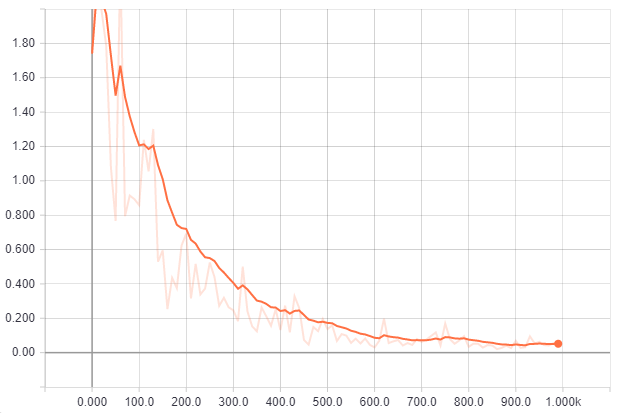
\includegraphics[width=\textwidth]{sections/experiments/loss_on_trainset}
	\caption{The step 1 loss of the training set as a function of the training steps.}
	\label{fig:train_loss}
\end{figure}

\begin{figure}
	\centering
	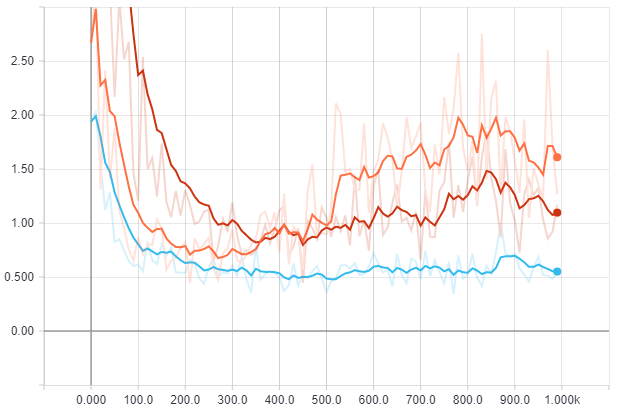
\includegraphics[width=\textwidth]{sections/experiments/regularization}
	\caption{The step 1 loss of the validation set as a function of the training steps.
	At the end off training is the top function without any regularization, 
	the second is with dropout and the last is with both drop out and 
	l2 regularization.}
	\label{fig:regularization}
\end{figure}

Some problems arose under training. In Figure \ref{fig:overfitting} is the loss of the 
validation set plotted as a function of the training steps, and it shows that the loss
stops improving at around training step 300, starts rising after that. The same trend 
cannot be seen in the loss on the training set as shown in Figure \ref{fig:train_loss}.
This is a sign of the model is overfitting by learning details about the training set 
that does not generalise to new data. Different techniques exists to prevent
overfitting. The two I have chosen to use is called dropout and l2 regularization.
With dropout a certain percentages of the output nodes of a layer is set to zero and 
the rest is scaled to keep the sum approximately the same. This forces the network 
to not rely on specific nodes and this helps reduce the overfitting. The other 
technique, l2 regularization, adds a term to the loss that is proportional to the sums 
of the weights. This prevents the weights from getting large which helps reduce the 
overfitting. In Figure \ref{fig:regularization} can the effect of the regularization
techniques be seen. The run where only dropout was used starts higher than the run where
no regularization was used but don't overfit as much so it ends below. The run with 
both dropout and l2 regularization starts below the other two and keeps below throughout 
the training and the problem of overfitting is also almost entirely gone. 

\subsection{Measurements}

\begin{figure}
	\centering
	
	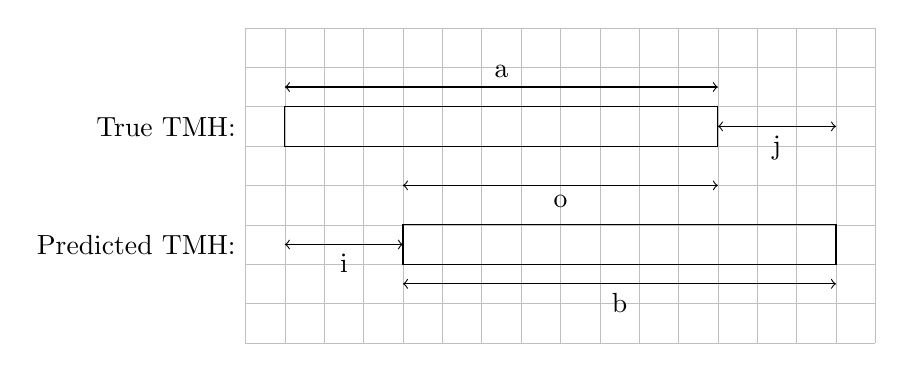
\begin{tikzpicture}[]
	\draw[step=0.5cm,very thin,color=lightgray] (0,-1) grid (8,3);
	
	\draw[] (0.5,1.5) rectangle (6,2);
	\node at (-0,1.5) [anchor=south east] {True TMH:};
	\draw[<->] (6,1.75) -- (7.5,1.75) node[pos=0.5, below]{j};
	\draw[<->] (0.5,2.25) -- (6,2.25) node[pos=0.5, above]{a};
	
	\draw[] (2,0) rectangle (7.5,0.5);
	\node at (-0,0) [anchor=south east] {Predicted TMH:};
	\draw[<->] (0.5,0.25) -- (2,0.25) node[pos=0.5, below]{i};
	\draw[<->] (2,-0.25) -- (7.5,-0.25) node[pos=0.5, below]{b};
	
	\draw[<->] (2,1) -- (6,1) node[pos=0.5, below]{o};
	\end{tikzpicture}
	
	\caption{Illustrations of used measurements in comparison of \glspl{tmh}. a is the length of true \gls{tmh},
		b is the length of the predicted \gls{tmh}, i is the difference in the start position, j is the difference
		in the end posetion and o is the length of the overlap.}
	\label{fig:thm_measurements}
\end{figure}

To evaluate the model some measure for the performance of the model have to be chosen.
I have chosen three different types of measurements that have three different purposes.
The loss function used in training of step 1 assigns a loss to each position with a 
wrong predicted class and the optimiser then tries to minimize this loss. 
Since the loss is calculated from each position, it seems apparent to also use a 
position based measurement. Especially to measure the performance of step 1.
This type of measurement does not see a \gls{tmh} as a single thing and can therefore
not say anything about the number of \glspl{tmh}. It is therefore also interesting 
to have a measure for this. I have used two different types of measurements to do this, 
both of them counts a consecutive sequence of positions classified as \gls{tmh} as a single
prediction. The purpose of step 1 was to identify regions with \glspl{tmh}.
The second measurement type's purpose is therefore to measure if a prediction of a 
\gls{tmh} is in the right region, this is done by finding the length of the overlap 
between the predicted \gls{tmh} and the true \gls{tmh}, denoted as $o$ in Figure 
\ref{fig:thm_measurements}, the length is then compared 
to the longest of the two \gls{tmh}. The predicted \gls{tmh} is counted as a correct prediction
if the ratio is larger than a certain value. This condition as an equation becomes:

\begin{equation}
	\frac{o}{\max(a, b)} \geq x
\end{equation}

Where $o$ is the length of the overlap, $a$ and $b$ is the length of the true \gls{tmh}
and the predicted \gls{tmh} respectively and $x$ is the minimum overlap ratio.
I have done this with different values to see how precise the predicted regions is. 

The last measurement type is intended to measure step 3. The purpose of
this step was to adjust the endpoints of predicted \glspl{tmh}, this measurement 
therefore looks at endpoints and counts a predicted \gls{tmh} as correct if both endpoints 
is within a certain number of positions of the true endpoints. 
As an equation this becomes:

\begin{equation}
	i \leq y \wedge j \leq y
\end{equation}

Where $i$ is the length between the start of the true \gls{tmh} and the predicted \gls{tmh},
$j$ is the length between the end of the two \gls{tmh} and $y$ is the maximum length these
differences can be. This is again done with 
different values for the allowed difference of endpoints. 

These two measurement types is derived from one of the measurement they use in TMSEG,
which is a combination of the two where the overlap have to be at least 50\% and the 
endpoints have to be within 5 positions of the true endpoints for a prediction to be counted
as correct. I have also used this measurement to be able to compare to the result they get 
there. 

For each condition for when a predicted \gls{tmh} is correct, precision and recall is calculated.
Precision is the percentages of the predicted \glspl{tmh} that is correct and recall is the 
percentages of true \glspl{tmh} that was correct predicted. Calculated the same way as in TMSEG:

\begin{align*}
	\text{Precision} &= \frac{\text{\# of correctly predicted TMHs}}{\text{\# of predicted TMHs}} * 100 \\
	\text{Recall} &= \frac{\text{\# of correctly predicted TMHs}}{\text{\# of true TMHs}} * 100
\end{align*}

